%! TeX program = lualatex

\documentclass[12pt]{report}
\usepackage[usenames,dvipsnames]{xcolor}
\usepackage{tcolorbox}
\usepackage[margin=1in]{geometry} 
\usepackage{amsmath,amsthm,amssymb}
\usepackage[english]{babel}
\usepackage[T1]{fontenc} %escribe lo del teclado
\usepackage[utf8]{inputenc} %Reconoce algunos símbolos
\usepackage{graphicx}
\usepackage{multirow}
\usepackage{wrapfig}
\usepackage{diagbox} %diagonal cells
\usepackage{dirtytalk}
\usepackage{caption}
\usepackage{subcaption}
\usepackage{minted}
\usepackage{booktabs}
\usepackage{import}
\usepackage{tikz}
\usepackage{pgfplots}
\usepackage{multicol}
\usetikzlibrary{arrows.meta}
\usetikzlibrary{fit}
\usepackage{hyperref}
\usepackage{titlesec} % To configure subsections

\titleformat*{\subsection}{\normalsize\bfseries}
\setcounter{tocdepth}{1} % Only sections
\definecolor{bg}{RGB}{240,240,240}
\newcolumntype{Z}{>{\ttfamily}{c}<{}}

\newcommand{\tbf}[1]{\textbf{\boldmath #1}}


\definecolor{mintedbackground}{rgb}{0.95,0.95,0.95}

% Font ligatures
\usepackage{fontspec}
\setmonofont[Contextuals={Alternate},Scale=0.8]{Fira Code}

\newmintedfile[cppcode]{cpp}{
bgcolor=mintedbackground,
linenos=true,
numberblanklines=true,
numbersep=5pt,
gobble=0,
frame=leftline,
framerule=0.4pt,
framesep=2mm,
funcnamehighlighting=true,
tabsize=4,
obeytabs=false,
mathescape=false
samepage=true, %with this setting you can force the list to appear on the same page
showspaces=false,
showtabs =false,
texcl=false,
fontsize=\small,
breaklines=true
}

\setminted[cpp]{
bgcolor=mintedbackground,
linenos=true,
numberblanklines=true,
numbersep=5pt,
gobble=0,
frame=leftline,
framerule=0.4pt,
framesep=2mm,
funcnamehighlighting=true,
tabsize=4,
obeytabs=false,
mathescape=false
samepage=true, %with this setting you can force the list to appear on the same page
showspaces=false,
showtabs =false,
texcl=false,
fontsize=\small,
breaklines=true
}

\begin{document}

\begin{titlepage}
    \begin{center}
        \vspace*{1cm}
 
        \Huge
        \textbf{Competitive Programming Algorithms}
 

 
        \vspace{1.5cm}
 
		\Large
        \textbf{David del Val}
 
        \vfill
 
 
        \vspace{0.8cm}
 
 
        \Large
	\today
 
    \end{center}
\end{titlepage}

\setcounter{tocdepth}{2}
\tableofcontents 
\chapter{Basic range queries }

\section{Types of range queries}
Depending on the type of function whose value we have to calculate over
the given range:
\begin{itemize}
		\item \textit{Idempotent functions}. These functions fulfill the 
				following condition $f(f(x))=f(x)$. For instance, the maximum
				and minimum of a list of values are idempotent. 
				Furthermore, since the GCD and LCM can be seen as 
				the \say{maximum} and the \say{minimum} of the exponents in the
				prime factorization, it is only natural that they fulfill the same 
				property.

				The most important property of these functions for range queries
				is that we can evaluate the elements of the range several times 
				without affecting the result. For instance:
				\[
						\min(a_l,\dots ,a_r)= \min \left (
								\min (a_l, \dots,  a_k), \min (a_{k},\dots, a_r)
						\right ) \quad l < k <r
				\]
				even though the union of the intervals includes $a_k$ twice.
				This is the property in which sparse tables are based.


		\item  \textit{Reversible functions}. Functions that have an inverse
				also have advantages in range queries. That is because we
				can easily remove elements from any range to obtain a smaller
				one. In these cases we can obtain the final range by adding
				and subtracting ranges that have been precalculated.

				For instance, the addition, subtraction and xor operations have 
				an inverse (subtraction, addition and xor respectively). 

\end{itemize}

\newpage
There are also other problems that can be transformed into a range query easily.

\subsection{LCA using RMQ}
To use this algorithm we need a rooted tree with undirected edges where the 
nodes are labeled in a particular order. Specifically, nodes at a greater
depth have to be labeled with a greater value. Furthermore, the algorithm
could be extended to process a forest (instead of a single tree) but 
this version cannot process forests.

We can traverse the tree using dfs and store in an array each node that we 
encounter. If we also keep track of the time at which each node was found
for the first time, the LCA can be converted into calculating the minimum
in an array of length $E+V$.

\begin{figure}[h!]
		\centering
		\resizebox{70 mm}{!}{\import{./figures/}{LCA_to_RMQ.pdf_tex}}
\end{figure}
After running a DFS in the tree, we would get the following array of 
values and discovery times:
\begin{figure}[h!]
		\centering
		\begin{subfigure}{0.55\textwidth}
		\centering
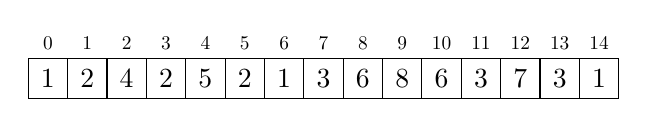
\begin{tikzpicture}
		\begin{scope}[shift={(-6,0)}]
				\foreach \m/\c in{
						0/1,
						1/2,
						2/4,
						3/2,
						4/5,
						5/2,
						6/1,
						7/3,
						8/6,
						9/8,
						10/6,
						11/3,
						12/7,
						13/3,
						14/1
				}{
				\pgfmathtruncatemacro{\om}{\m}
				\pgfmathsetmacro{\sm}{0.5*\m}
				\pgfmathsetmacro{\em}{0.5+\sm}
				\node[draw, fit={(\sm,0)(\em,0.5)}, inner sep = 0 pt, label = center: \c](A){};
				\node[fit={(\sm,0.6)(\em,0.8)}, inner sep = 0 pt, label = center: \scalebox{0.7}{\om}](A){};
				}
		\end{scope}
\end{tikzpicture}
		\end{subfigure}
		\begin{subfigure}{0.4\textwidth}
		\centering
		\scalebox{0.9}{
				\begin{tabular}{c|c||c|c}
						\footnotesize{ \textbf{Node}} & \footnotesize{\textbf{Time}}&
						\footnotesize{\textbf{Node}} & \footnotesize{\textbf{Time}}\\
						\hline \hline
						1 & 0 &5 & 4\\
						2 & 1 &6 & 8\\
						3 & 7 &7 & 12\\
						4 & 2 &8 & 9\\
				\end{tabular}
		}
		\end{subfigure}

\end{figure}

Now if we want to get the LCA between nodes 5 and 6, we have to obtain the minimum
value in the range [4, 8]. As we can see, the result is obviously 1.

If we compare this approach to binary lifting, we observe that we have a considerably
more expensive precalculation phase but, afterwards, answering any queries takes
constant time instead of logarithmic time. In particular, the complexities for this 
method are:
\begin{itemize}
		\setlength{\itemsep}{1pt}
		\item Precomputate the values: $\mathcal{O}(E\log(E))$
		\item Calculate the LCA of a node: $\mathcal{O}(1)$
		\item Memory usage: $\mathcal{O}(E\log(E))$
\end{itemize}
Where $E=\text{edges}$.

\newpage


\section{Sparse table}
The sparse table is a data structure that calculates the value of 
a function over a range of immutable elements with the following complexity:
\begin{itemize}
		\setlength{\itemsep}{2 pt}
		\item \tbf{$\mathcal O(n\log n)$} to build the data structure
		\item \tbf{$\mathcal O(1)$} to answer queries on a range. 
		\item \tbf{$\mathcal O(n\log n)$} memory
\end{itemize}
Furthermore, the function must be \textbf{idempotent}. This allows the use of
overlapped intervals in the calculations. A Sparse Table can be adapted to 
answer queries with more general functions. However, it would lose the constant
time query capabilities and would be no more efficient than a segment tree or a BIT.


On the other hand, the data structure is rather simple and its implementation 
is considerable shorter than any other alternatives. 

The table consists of $\log n$ rows. Each one of them contains the value of the
function in intervals of length $2^j$ where $j$ is the row index. In particular,
table$[j][i]=f([i,i+2^j])$, where $f(I)$ is the value of $f$ over all the 
elements in $I$.

To construct the table we take advantage of the fact that the intervals of each
row are the exact union of two intervals of the previous row. Additionally, we 
have to create a lookup table for logarithms so that the queries can be 
processed fast enough.
It is important to notice that if many sparse tables where to be constructed,
it would be advisable to share the log array among them by populating it with
all the values that might be needed initially or using a DP recursive approach.

\newpage
\subsection{Example}
One of the best applications of the sparse table is to calculate the maximum of 
any range in an array of elements. The following illustration displays all the 
intervals that will be included in the sparse table. To avoid intersections, 
intervals that belong to the same level of the table may be displayed above 
or below each other.

In each interval, we can see both the index (top left corner) and the value of
the maximum in that interval. It can also be seen that all intervals can 
be calculated using the values obtained in the previous level.
\begin{figure}[h!]
		\centering

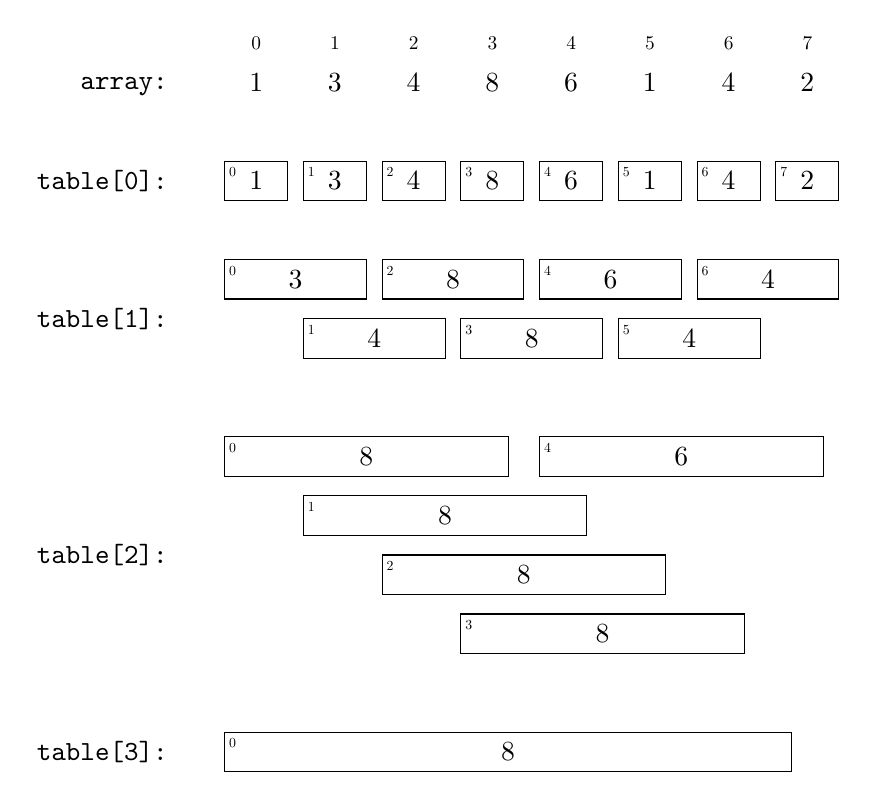
\begin{tikzpicture}
		\begin{scope}
				\foreach \m/\c in{
						0/1,
						1/3,
						2/4,
						3/8,
						4/6,
						5/1,
						6/4,
						7/2
				}{
				\pgfmathtruncatemacro{\om}{\m}
				\pgfmathsetmacro{\sm}{1*\m}
				\pgfmathsetmacro{\em}{1+\sm}
				\node[fit={(\sm,0.9)(\em,1.1)}, inner sep = 0 pt, label = center: \scalebox{0.7}{\om}](A){};
				\node[fit={(\sm,0.25)(\em,0.75)}, inner sep = 0 pt, label = center: \c](A){};
				}
		\end{scope}
		\begin{scope}
				\foreach \i/\c in 
				{
						0/1,
						1/3,
						2/4,
						3/8,
						4/6,
						5/1,
						6/4,
						7/2
				}
				{
				\pgfmathsetmacro{\sm}{0.1+1*\i}
				\pgfmathsetmacro{\lm}{0.1+1*\i+0.2}
				\pgfmathsetmacro{\em}{0.8+\sm}
				\node[fit={(\sm,-0.9)(\lm,-0.5)}, inner sep = 0 pt, ](A){\scalebox{0.5}{\i}};
				\node[draw, fit={(\sm,-1)(\em,-0.5)}, inner sep = 0 pt, label = center: \c](A){};
				}

				\foreach \i/\c/\m in 
				{
						0/3/0,
						1/4/1,
						2/8/0,
						3/8/1,
						4/6/0,
						5/4/1,
						6/4/0
				}
				{
				\pgfmathsetmacro{\sm}{0.1+1*\i}
				\pgfmathsetmacro{\lm}{0.1+1*\i+0.2}
				\pgfmathsetmacro{\em}{1.8+\sm}
				\pgfmathsetmacro{\sh}{-2.25-\m*0.75}
				\pgfmathsetmacro{\lh}{0.1+\sh}
				\pgfmathsetmacro{\eh}{0.5+\sh}

				\node[fit={(\sm,\lh)(\lm,\eh)}, inner sep = 0 pt, ](A){\scalebox{0.5}{\i}};
				\node[draw, fit={(\sm,\sh)(\em,\eh)}, inner sep = 0 pt, label = center: \c](A){};
				}

				\foreach \i/\c/\m in 
				{
						0/8/0,
						1/8/1,
						2/8/2,
						3/8/3,
						4/6/0
				}
				{
				\pgfmathsetmacro{\sm}{0.1+1*\i}
				\pgfmathsetmacro{\lm}{\sm+0.2}
				\pgfmathsetmacro{\em}{3.6+\sm}
				\pgfmathsetmacro{\sh}{-4.5-\m*0.75}
				\pgfmathsetmacro{\lh}{0.1+\sh}
				\pgfmathsetmacro{\eh}{0.5+\sh}

				\node[fit={(\sm,\lh)(\lm,\eh)}, inner sep = 0 pt, ](A){\scalebox{0.5}{\i}};
				\node[draw, fit={(\sm,\sh)(\em,\eh)}, inner sep = 0 pt, label = center: \c](A){};
				}

				\foreach \i/\c/\m in 
				{
						0/8/0
				}
				{
				\pgfmathsetmacro{\sm}{0.1+1*\i}
				\pgfmathsetmacro{\lm}{\sm+0.2}
				\pgfmathsetmacro{\em}{7.2+\sm}
				\pgfmathsetmacro{\sh}{-8.25-\m*0.75}
				\pgfmathsetmacro{\lh}{0.1+\sh}
				\pgfmathsetmacro{\eh}{0.5+\sh}

				\node[fit={(\sm,\lh)(\lm,\eh)}, inner sep = 0 pt, ](A){\scalebox{0.5}{\i}};
				\node[draw, fit={(\sm,\sh)(\em,\eh)}, inner sep = 0 pt, label = center: \c](A){};
				}

				\node[anchor=east] (a) at (-0.5,0.45){\texttt{array:}};
				\node[anchor=east] (a) at (-0.5,-0.75){\texttt{table[0]:}};
				\node[anchor=east] (a) at (-0.5,-2.5){\texttt{table[1]:}};
				\node[anchor=east] (a) at (-0.5,-5.5){\texttt{table[2]:}};
				\node[anchor=east] (a) at (-0.5,-8){\texttt{table[3]:}};

		\end{scope}
		\end{tikzpicture}
\end{figure}

\noindent
Now, if we want to calculate the maximum between indices 2 and 7 we will:
\begin{enumerate}
		\setlength{\itemsep}{2pt}
		\item Calculate the length of the interval. In this case, $7-2+1=6$
		\item Calculate the maximum value of $k$  such that $2^k<6$. In this
				case, $k=2$.
		\item Pick the interval that starts on 2 with length $2^k=4$ and the
				interval that starts on $7-2^k+1$ with the same length. 
				That is to say, intervals 2 and 4 from level 2 of the table.

				As we can see these intervals cover the entire range, albeit 
				they overlap. However, the overlap does not affect the result
				of the maximum.
		\item Take the maximum between the values of the two intervals 
				selected: $\max(8,6)=8$
\end{enumerate}

\newpage
\cppcode[firstline=20]{code/data_structures/SparseTable.cpp}
\newpage

\subsection{Sparse Table with $\mathcal{O}(n)$ memory}

This variant of the sparse table is only capable of answering very
specific queries. In particular, the operation must meet the following
constraints:
\begin{itemize}
		\setlength{\itemsep}{2pt}
		\item It is idempotent (as in a normal Sparse Table)
		\item The result of the operation over a range is an element
				in that range
\end{itemize}
Therefore, this data structure will mostly only be used for querying the
maximum or the minimum over a range. On the other hand, we obtain a data 
structure that uses significantly less memory and can be built in
considerably less time, albeit with slower queries.

\cppcode[firstline=20]{code/data_structures/Linear_RMQ.cpp}
With that goal in mind, we will group the 


\begin{figure}[h!]
		\centering
		\resizebox{\textwidth}{!}{\import{./figures/}{Optimized_Sparse.pdf_tex}}
\end{figure}

\newpage
\section{Fenwick tree (BIT)}
A Fenwick tree or binary indexed tree (BIT) can be used to calculate the value
of a \textbf{reversible} function $F$ over a range of values. Given an array of elements
$A$ of size $N$:
\begin{itemize}
		\setlength{\itemsep}{2pt}
		\item Given a range $[l,r]$, the value $F(a_l,\dots, a_r)$ can be calculated
				in \tbf{$\mathcal{O}(\log n)$}
		\item Updating one of the values of the array takes \tbf{$\mathcal{O}(\log n)$}
		\item Requires the same amout of memory as the array $A$
\end{itemize}
To do so, we create a new array \texttt{ft} where each element represents
the value of the function over a particular range. Let LSOne($i$) be the 
result of setting to 0 all bits of $i$ except for the least significant one.
For instance, LSOne$(0110)=0010$. Then, the $i$-th element of \texttt{ft} 
contains the value $F(a_{i-\text{LSOne}(i)+1},\dots, a_{i})$. 

In most cases, $F$ will be the sum of all elements $F(a_l,\dots, a_r)=\sum_l^r{a_i}$.
In that case, \text{ft[i]} contains the sum of all the elements from 
position $i-\text{LSOne}(i)$ (excluded) to position $i$ (included).


It is also important to note that this BIT is \textbf{1-indexed interally} to simplify slightly 
the implementation. However, the interface automatically subtracts one to all index parameters
given.
\subsection*{Range Update and Point Query}
The standard BIT allows point update and range query. Using a difference array, we can 
transform them into range update and point query. If $B$ is the difference array
of $A$, the elements of $B$ are defined as:  $b_i=a_i- a_{i-1}$ and $b_1=a_1$.
Therefore:
\begin{itemize}
		\setlength{\itemsep}{2pt}
		\item $\sum_{1}^i b_j=a_i$, converting the range query into 
				a point query
		\item To update the elements in the range $[l,r]$ by $d$, we can add
				$d$ to the $l$-th element and subtract $d$ from the $r$-th element.
				In doing so, queries that reach until a point
				between $l$ and $r$ will be increased by $d$ but queries that reach 
				further will not be affected.
				Therefore we have converted two point updates into a range update.

\end{itemize}

\subsection*{Example}
For instance, if we use the addition operation, array on the left would be processed
into the BIT tree displayed on the right. Each box under the BIT tree represents
the elements that are added to get the value of that position.
\begin{figure}[h!]
		\centering
		\scalebox{0.85}
		{
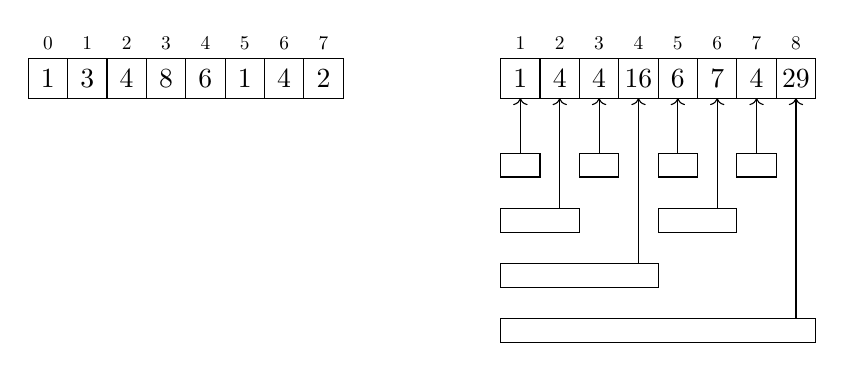
\begin{tikzpicture}
		\begin{scope}[shift={(-6,0)}]
				\foreach \m/\c in{
						0/1,
						1/3,
						2/4,
						3/8,
						4/6,
						5/1,
						6/4,
						7/2
				}{
				\pgfmathtruncatemacro{\om}{\m}
				\pgfmathsetmacro{\sm}{0.5*\m}
				\pgfmathsetmacro{\em}{0.5+\sm}
				\node[draw, fit={(\sm,0)(\em,0.5)}, inner sep = 0 pt, label = center: \c](A){};
				\node[fit={(\sm,0.6)(\em,0.8)}, inner sep = 0 pt, label = center: \scalebox{0.7}{\om}](A){};
				}
		\end{scope}
		\begin{scope}
				\foreach \m/\c in{
						0/1,
						1/4,
						2/4,
						3/16,
						4/6,
						5/7,
						6/4,
						7/29
				}{
				\pgfmathtruncatemacro{\om}{\m+1}
				\pgfmathsetmacro{\sm}{0.5*\m}
				\pgfmathsetmacro{\em}{0.5+\sm}
				\node[draw, fit={(\sm,0)(\em,0.5)}, inner sep = 0 pt, label = center: \c](A){};
				\node[fit={(\sm,0.6)(\em,0.8)}, inner sep = 0 pt, label = center: \scalebox{0.7}{\om}](A){};
				}
				\draw (0, -1) rectangle ++(0.5,0.3);
				\draw [->] (0.25,-0.7)--(0.25,0);
				\draw (1, -1) rectangle ++(0.5,0.3);
				\draw [->] (1.25,-0.7)--(1.25,0);
				\draw (2, -1) rectangle ++(0.5,0.3);
				\draw [->] (2.25,-0.7)--(2.25,0);
				\draw (3, -1) rectangle ++(0.5,0.3);
				\draw [->] (3.25,-0.7)--(3.25,0);

				\draw (0, -1.7) rectangle ++(1.0,0.3);
				\draw [->] (0.75,-1.4)--(0.75,0);

				\draw (2, -1.7) rectangle ++(1.0,0.3);
				\draw [->] (2.75,-1.4)--(2.75,0);

				\draw (0, -2.4) rectangle ++(2.0,0.3);
				\draw [->] (1.75,-2.1)--(1.75,0);

				\draw (0, -3.1) rectangle ++(4.0,0.3);
				\draw [->] (3.75,-2.8)--(3.75,0);

		\end{scope}
\end{tikzpicture}
}
\end{figure}

\newpage
\cppcode[firstline=20]{code/data_structures/BIT.cpp}



\chapter{Graphs}

\section{Dijkstra's}
Shortest path from \texttt{orig} node to \texttt{dest} (or to every node) in a graph
that does not contain negative edges. 
It chooses the best path greedily in each iteration and, therefore, it only works
on graphs without negative weights. 
\cppcode[firstline=20]{code/graph/dijkstra.cpp}
\noindent \textbf{\boldmath Running time: $\mathcal{O}(E+V\log V)$}
\\ {\small(V = vertices, E = edges)}
\subsection*{Remarks}
\begin{itemize}
	\item If we ignore the check in line 30, we can return the distances 
		vector, which will contain the shortest distance from \texttt{dist}
		to every other node.
	\item If we are doing some kind of pruning it is imperative that we prune 
	as many branches as possible in the main loop. That is to say, we should
	introduce as many \texttt{if} statements in line 36 to make sure that we
	run the \texttt{for} loop as few times as possible. 

	An example of this approach is problem \texttt{UVA-11635}. In that problem, we
	add a lot of branches to the queue (we may run the \texttt{for} loop
	twice in some nodes) but we prune them in the main loop. Thus the 
	running time is still acceptable.

\item  However, pruning the branches with a higher cost can be quite complicated 
	when we have to optimize several factors (see section \ref{graph:dijkstra:distances}).
	Therefore, we will omit the check in line \texttt{33} if we think it might discard 
	relevant options.

\end{itemize}

\newpage
\subsection{Dijkstra with cost and distance}
\label{graph:dijkstra:distances}
In this problem we are going to define two values for each edge, cost and distance:
\begin{itemize}
	\setlength\itemsep{0 pt}
	\item \textit{Cost}. This is the number that we want to minimize. It is the 
		equivalent to the usual cost in a normal Dijkstra problem
	\item \textit{Distance}. We define the distance of a path as the sum of the
		distances of the edges in it. And the distance of the path from source
		to destination cannot exceed a given limit (\texttt{B})
\end{itemize}
This problem can be solved with a slightly modified version of Dijkstra's:
\cppcode[firstline=20]{code/graph/dijkstra_2.cpp}
\noindent \textbf{\boldmath Running time: $\mathcal{O}\big(B\cdot(V+E\log E)\big)$}
\\ {\small(V = vertices, E = edges, B = max\_distance)}

In this algorithm, we will process each node at most \texttt{B} times. Furthermore, 
if we process a node with a cost $c$ and a distance $d$, we know that this is the 
best possible cost for that distance $d$ since all the nodes in the queue have a higher
cost already. Therefore, we can close the node for that particular distance value (line 37).

An example of this algorithm is \texttt{SWERC-19\_20-A}


\section{Bellman Ford's}
Shortest parth from \texttt{orig} to every other node. It is slower than Dijkstra but 
it works on graphs with negative weights. 

This algorithm works by trying to relax every edge $V-1$ times. If there are no 
negative cycles, after $V-1$ iterations, we must have found the minimum distance
to every node. Therefore if after these iterations, we run another
iteration and the distance to a node decreases, we must have a negative cycle.

\cppcode[firstline=20]{code/graph/bellman_ford.cpp}
\noindent \textbf{\boldmath Running time: $\mathcal{O}(VE)$}
\\ {\small(V = vertices, E = edges)}
\subsection*{Remarks}
\begin{itemize}
	\item If we keep track of the distance that decrease when we check for
		a negative cycle, we will get at least one node of 
		every negative cycle present in the graph.

		We can use this, for instance, to check if we can reach a node with 
		a cost smaller than a given bound. If it is connected to a node in a 
		negative cycle, it's distance will be as small as we want it to be
		(by looping in the cycle).

		This can be seen at play in \texttt{UVA-10557}
		\newpage
	\item If we modify slightly the main loop, iteration $i$ will be the 
		result of considering paths of at most $i+1$ edges:
		\begin{minted}{cpp}
for (int i = 0; i < n - 1; ++i) {
        for (auto e : edges) {
            dists2[e.fi.se] = min(dists2[e.fi.se], dists[e.fi.fi] + e.se);
        }
	dists = dists2;
}
		\end{minted}
		This can be seen at play in \texttt{UVA-11280}
		

\end{itemize}	

\section{Warshall's}
Warshall's algorithm solves the APSP (All pairs shortest path) using DP.
Each iteration of the outer loop tries to add a node (the $k$-th node in
particular) to the path between all pairs of nodes. 
We can think of the comparison as: 
\begin{center}
		\textit{ Is the path from $i$ to $j$ shorter if we first 
		move from $i$ to $k$ and, then, from $k$ to $j$? }
\end{center}
It is important to note that we must use an adjacency matrix in this
implementation.
\cppcode[firstline=20]{code/graph/basicWarshall.cpp}
\noindent \textbf{\boldmath Running time: $\mathcal{O}(V^3)$}
\\ {\small (V = vertices, E = edges)}
\subsubsection*{Obtaining the path}
To get the explicit path, we will store the last vertex in the 
path that the algorithm found to go from $i$ to $j$. That is to say,
after  a given iteration the optimal path from $i$ to $j$ is:
\begin{figure}[h!]
		\centering
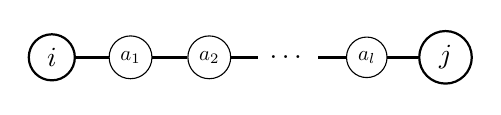
\begin{tikzpicture}
	\begin{scope}[every node/.style = {circle, thick, draw}]
		\node (A) at (0,0) {$i$};
		\node (C) at (5,0) {$j$};
	\end{scope}
	\begin{scope}[every node/.style = {scale=0.75, circle,   draw}]
		\node (B1) at (1,0) {$a_1$};
		\node (B2) at (2,0) {$a_2$};
		\node (E2) at (4,0) {$a_{l}$};
	\end{scope}
	\begin{scope}[every node/.style = { circle   }]
		\node (D) at (3,0) {$\dots$};
	\end{scope}
	\begin{scope}[>={Stealth[black]},
			every edge/.style={draw=black, very thick}]
		\path [-] (A) edge  (B1);
		\path [-] (B1) edge  (B2);
		\path [-] (B2) edge  (D);
		\path [-] (D) edge  (E2);
		\path [-] (E2) edge  (C);
	\end{scope}
\end{tikzpicture}
\end{figure}
Then we should store that the last node in the path that goes from $i$
to $j$ is $a_j$. 
The code to do so is the following:
\cppcode[firstline=20]{code/graph/pathWarshall.cpp}
\newpage




\section{DFS}
\subsection{Articulation points and bridges}
These algorightms can be used in undirected graphs, and we
will use the following definitions:
\begin{itemize}
	\def\itemsep{0 pt}
	\item \textbf{Articulation point}. A node whose removal would increase the number
		of connected components of the graph. That  is to say
		that it \say{splits} a connected component.
	\item \textbf{Bridge}. An edge whose removal increases the number of 
		connected components in the graph.
\end{itemize}
We will use a modified version of DFS to solve this problem. We mainly introduce two new
properties for every node:
\begin{itemize}
	\def\itemsep{0 pt}
	\item \texttt{num}. Time at which the node was first explored by DFS
	\item \texttt{low}. Earliest node that can be found in the DFS spanning 
		tree that starts from this node
\end{itemize}
When we visit a node, for every edge, there are two options:
\begin{itemize}
\def \itemsep{0pt}
	\item \textbf{Tree edge}. This edge point to a node that has not been 
		discovered yet. As such we explore it (calling \texttt{dfs})
		and, we update the value of \texttt{low} for the current
		node. 

		After the update, we can now process the child since we will
		not visit it again and it's DFS tree has been fully explored

	\item \textbf{Back edge}. This edge points to a node that has already
		been visited. Therefore, it will have a relatively low 
		\texttt{num} and we use it to update the \texttt{low}
		value of the current node
\end{itemize}
\newpage
\cppcode[firstline=20]{code/graph/articulationPts.cpp}
\noindent \textbf{\boldmath Running time: $\mathcal{O}(V+E)$}
\\ {\small (V = vertices, E = edges)}
\subsubsection*{Explanation}

The first graph that we will consider is the following:
\begin{figure}[h]
\centering
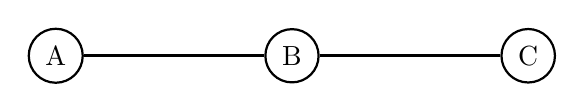
\begin{tikzpicture}
	\begin{scope}[every node/.style = {circle, thick, draw}]
		\node (A) at (0,0) {A};
		\node (B) at (3,0) {B};
		\node (C) at (6,0) {C};
	\end{scope}
	\begin{scope}[>={Stealth[black]},
			every edge/.style={draw=black, very thick}]
		\path [-] (A) edge  (B);
		\path [-] (B) edge  (C);
	\end{scope}
\end{tikzpicture}
\end{figure}
After applying DFS on $A$ we get the following DFS spanning tree.
Above every node, we have included \texttt{num / low}.
\begin{figure}[h]
\centering
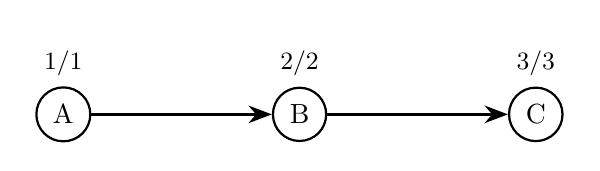
\begin{tikzpicture}
	\begin{scope}[every node/.style = {circle, thick, draw},
		every label/.append style={font = \small, yshift = -0.5 em}]
		\node[label={1/1}] (A) at (0,0) {A};
		\node[label={2/2}](B) at (3,0) {B};
		\node[label={3/3}](C) at (6,0) {C};
	\end{scope}
	\begin{scope}[>={Stealth[black]},
			every edge/.style={draw=black, very thick}]
		\path [->] (A) edge  (B);
		\path [->] (B) edge  (C);
	\end{scope}
\end{tikzpicture}
\end{figure}

This is a rather simple graph and it's only articulation point is $B$. This is because
it has a child whose \texttt{low} value is greater than or equal to $B$'s  \texttt{num}
value. Therefore, there is no connection from that child (namely $C$) to a node explored
before $B$ that does not go through $B$. 

However, we can already see that the root has to be treated as a separate case. 
The root will be an articulation point iff it has more than one child in its DFS tree. 
It is important to note that the children of the DFS tree need not be the same as the 
children of the root in the initial graph.

Let's look at another example
\begin{figure}[h]
\centering
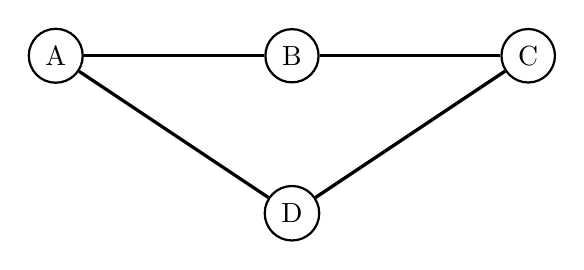
\begin{tikzpicture}
	\begin{scope}[every node/.style = {circle, thick, draw},
		every label/.append style={font = \small, yshift = -0.5 em}]
		\node (A) at (0,0) {A};
		\node (B) at (3,0) {B};
		\node (C) at (6,0) {C};
		\node (D) at (3,-2) {D};
	\end{scope}
	\begin{scope}[>={Stealth[black]},
			every edge/.style={draw=black, very thick}]
		\path [-] (A) edge  (B);
		\path [-] (B) edge  (C);
		\path [-] (C) edge  (D);
		\path [-] (D) edge  (A);
	\end{scope}
\end{tikzpicture}
\end{figure}

As before, we show the DFS spanning tree:
\begin{figure}[h!]
\centering
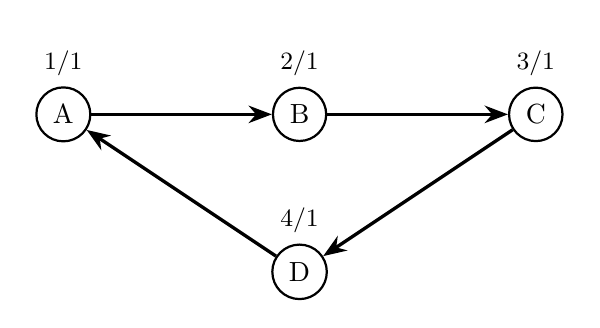
\begin{tikzpicture}
	\begin{scope}[every node/.style = {circle, thick, draw},
		every label/.append style={font = \small, yshift = -0.5 em}]
		\node [label={1/1}] (A) at (0,0) {A};
		\node [label={2/1}](B) at (3,0) {B};
		\node [label={3/1}](C) at (6,0) {C};
		\node [label={4/1}](D) at (3,-2) {D};
	\end{scope}
	\begin{scope}[>={Stealth[black]},
			every edge/.style={draw=black, very thick}]
		\path [->] (A) edge  (B);
		\path [->] (B) edge  (C);
		\path [->] (C) edge  (D);
		\path [->] (D) edge  (A);
	\end{scope}
\end{tikzpicture}
\end{figure}

Now we have no articulation point since there is no node that has a child
with a \texttt{low} greater than or equal  than the parent's \texttt{num}. 
This difference is caused by the fact that now there is an edge that makes $C$
accessible through a path that does not involve traversing $B$.

In this case, we can see how the root has only one child in the spanning tree
but two in the initial graph. This reflects the fact that those numbers need not
coincide.

Finally, the condition for a bridge is: \texttt{low[child]>num[parent]}. This is 
equivalent to  stating that the child has no other way of reaching either the
parent or a node that was explored before the parent

\subsection{Trajan's algorithm for strongly connected components}
In a directed graph, we say that a subset of vertices comprises a strongly 
connected component if every vertex is reachable from every other vertex in
this subset.

We will now present an algorithm that divides the graph into strongly
connected parts that are as large as possible. It will use some of the 
same concepts as in the previous section. 
\subsubsection*{Explanation}
The main idea is the following: if when we are done with a node, we have not been
able to reach a node that was further back, this one is the root of a SCC. 

Let's explain this reasoning with an example:

\begin{figure}[h]
\centering
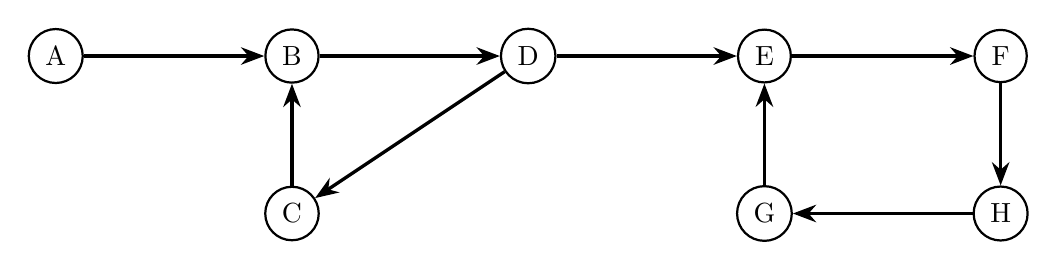
\begin{tikzpicture}
	\begin{scope}[every node/.style = {circle, thick, draw},
		every label/.append style={font = \small, yshift = -0.5 em}]
		\node (A) at (0,0) {A};
		\node (B) at (3,0) {B};
		\node (C) at (3,-2) {C};
		\node (D) at (6,0) {D};
		\node (E) at (9,0) {E};
		\node (F) at (12,0) {F};
		\node (G) at (9,-2) {G};
		\node (H) at (12,-2) {H};
	\end{scope}
	\begin{scope}[>={Stealth[black]},
			every edge/.style={draw=black, very thick}]
		\path [->] (A) edge  (B);
		\path [<-] (B) edge  (C);
		\path [<-] (C) edge  (D);
		\path [->] (B) edge  (D);
		\path [->] (D) edge  (E);
		\path [->] (E) edge  (F);
		\path [->] (F) edge  (H);
		\path [->] (H) edge  (G);
		\path [->] (G) edge  (E);
	\end{scope}
\end{tikzpicture}
\end{figure}
And, after running DFS, we would get the following 
spanning tree with three SCCs.

\begin{figure}[h]
\centering
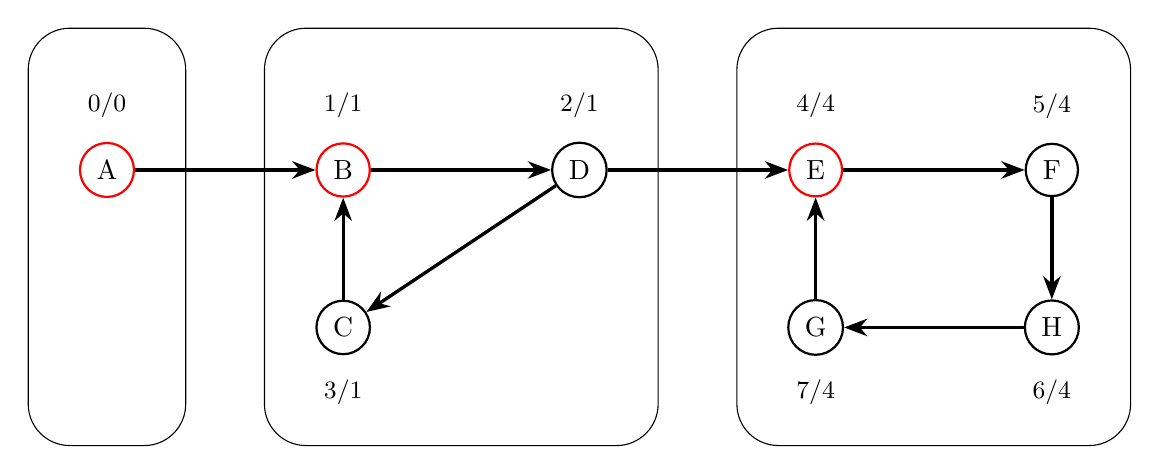
\begin{tikzpicture}
	\begin{scope}[every node/.style = {circle, thick, draw},
		every label/.append style={font = \small}]
		\node[label={0/0},draw=red] (A) at (0,0) {A};
		\node[label={1/1},draw=red] (B) at (3,0) {B};
		\node[label=below:{3/1}] (C) at (3,-2) {C};
		\node[label={2/1}] (D) at (6,0) {D};
		\node[label={4/4},draw=red] (E) at (9,0) {E};
		\node[label={5/4}] (F) at (12,0) {F};
		\node[label=below:{7/4}] (G) at (9,-2) {G};
		\node[label=below:{6/4}] (H) at (12,-2) {H};
	\end{scope}
	\begin{scope}[>={Stealth[black]},
			every edge/.style={draw=black, very thick}]
		\path [->] (A) edge  (B);
		\path [<-] (B) edge  (C);
		\path [<-] (C) edge  (D);
		\path [->] (B) edge  (D);
		\path [->] (D) edge  (E);
		\path [->] (E) edge  (F);
		\path [->] (F) edge  (H);
		\path [->] (H) edge  (G);
		\path [->] (G) edge  (E);
	\end{scope}
\draw[rounded corners=15pt] (-1,-3.5) rectangle ++(2,5.3);
\draw[rounded corners=15pt] (2,-3.5) rectangle ++(5,5.3);
\draw[rounded corners=15pt] (8,-3.5) rectangle ++(5,5.3);
\end{tikzpicture}
\end{figure}

Let's look  at the moment in which we close node $F$. As we can see the \texttt{low}
value is lower than the \texttt{num}. Therefore, there is a connection from $F$ to
another node that was visited before and it will be a part of the SCC \say{generated}
by that node.

However, when we close $E$, we can see that the \texttt{low} and the \texttt{num}
are equal. As a result, there is no way to get to a node that has a number lower than
E's through the spanning tree of $E$. Therefore, there is no way to have a bigger 
SCC that contains $E$.

To get the nodes that are part of the SCC, we need to get all the nodes in the stack before
the one that \say{generates} the SCC ($g$). This is because the stack only contains the 
nodes that belong to the spanning tree of $g$ and do not belong to any other SCC. 
Therefore, they must belong to the one generated by $g$. 

Furthermore, all those nodes will have the same \texttt{low} value since the \texttt{low}
any node with a higher value must have been processed before. Therefore, $g$ is accessible
from all those nodes and, clearly, all those nodes are accessible from $g$.
Thus, they fulfill the definition of an SCC.



\newpage
\cppcode[firstline=20]{code/graph/trajanSCC.cpp}
\noindent \textbf{\boldmath Running time: $\mathcal{O}(V+E)$}
\\ {\small (V = vertices, E = edges)}

\section{Kosaraju's}
Kosaraju's algorithm is a slightly simpler method for finding the SCC of a graph. 
On the other hand, it is also somewhat slower than Trajan's approach since it will
require running DFS on the graph twice. The algorithm follow this procedure:
\begin{enumerate}
	\item Run DFS on the graph and store the vertices in postorder in a list 
		called \texttt{postorder}.
	\item Reverse the graph
	\item Loop through the nodes in \texttt{postorder} starting from the one that 
		was closed the last. For each of them check if it has already been 
		added to a SCC (visited). If it hasn't, run DFS from that node and
		create a SCC with all the nodes that this DFS visits and hadn't been
		visited before.
\end{enumerate}
\subsubsection{Example}
Let's look at an example graph where we have run DFS starting first in node 
$A$ and, since it didn't explore the entire graph, we also run it from node $C$.
We have included the time at which each node was closed:
\begin{figure}[h]
\centering
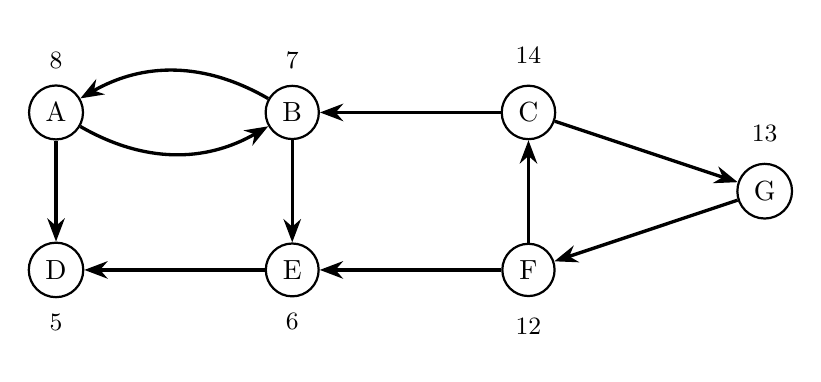
\begin{tikzpicture}
	\begin{scope}[every node/.style = {circle, thick, draw},
		every label/.append style={font = \small}]
		\node [label=8] (A) at (0,0) {A};
		\node [label=7] (B) at (3,0) {B};
		\node [label=14] (C) at (6,0) {C};
		\node [label=below:5] (D) at (0,-2) {D};
		\node [label=below:6] (E) at (3,-2) {E};
		\node [label=below:12] (F) at (6,-2) {F};
		\node [label=13] (G) at (9,-1) {G};
	\end{scope}
	\begin{scope}[>={Stealth[black]},
			every edge/.style={draw=black, very thick}]
		\path [->] (A) edge[bend right=30] (B);
		\path [->] (A) edge (D);
		\path [->] (B) edge[bend right=30] (A);
		\path [->] (B) edge (E);
		\path [->] (C) edge (B);
		\path [->] (C) edge (G);
		\path [->] (F) edge (C);
		\path [->] (F) edge (E);
		\path [->] (G) edge (F);
		\path [->] (E) edge (D);
	\end{scope}
\end{tikzpicture}
\end{figure}

Now we reverse the graph and we get the following:
\begin{figure}[h]
\centering
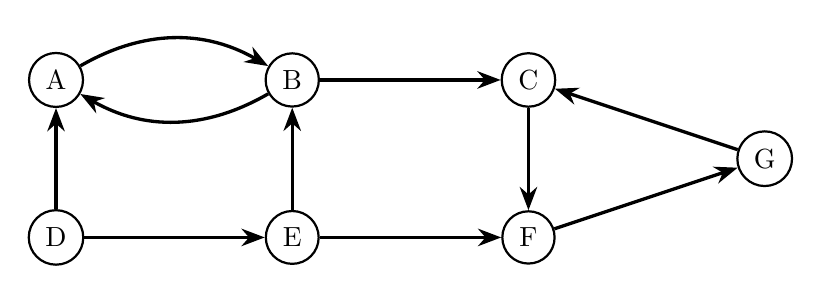
\begin{tikzpicture}
	\begin{scope}[every node/.style = {circle, thick, draw},
		every label/.append style={font = \small}]
		\node (A) at (0,0) {A};
		\node (B) at (3,0) {B};
		\node (C) at (6,0) {C};
		\node (D) at (0,-2) {D};
		\node (E) at (3,-2) {E};
		\node (F) at (6,-2) {F};
		\node (G) at (9,-1) {G};
	\end{scope}
	\begin{scope}[>={Stealth[black]},
			every edge/.style={draw=black, very thick}]
		\path [<-] (A) edge[bend right=30] (B);
		\path [<-] (A) edge (D);
		\path [<-] (B) edge[bend right=30] (A);
		\path [<-] (B) edge (E);
		\path [<-] (C) edge (B);
		\path [<-] (C) edge (G);
		\path [<-] (F) edge (C);
		\path [<-] (F) edge (E);
		\path [<-] (G) edge (F);
		\path [<-] (E) edge (D);
	\end{scope}
\end{tikzpicture}
\end{figure}


Finally, we can loop through the nodes in postorder, starting with the node
that was close the last:
\[
	\mathrm{postorder}=\{C,G,F,A,B,E,D\}
\]
\newpage
\begin{enumerate}
\def \itemsep{0pt}
	\item We run DFS on node $C$ and we get the SCC:
		\[
			s_1=\{C,F,G\}
		\]
	\item We skip nodes $G$ and $F$ in the list since they are already in
		a SCC and we run DFS on node $A$, getting the SCC:
		\[
			s_2=\{A,B\}	
		\]

	\item We skip node $B$ since it is already in a SCC and we 
		run DFS on node $E$, getting the SCC:
		\[
			s_3=\{E\}
		\]
	\item We finally run DFS on node $D$, and we get the last SCC:
		\[
			s_4=\{D\}
		\]
\end{enumerate}
Now, returning to the initial graph, we have found the following SCCs:

\begin{figure}[h]
\centering
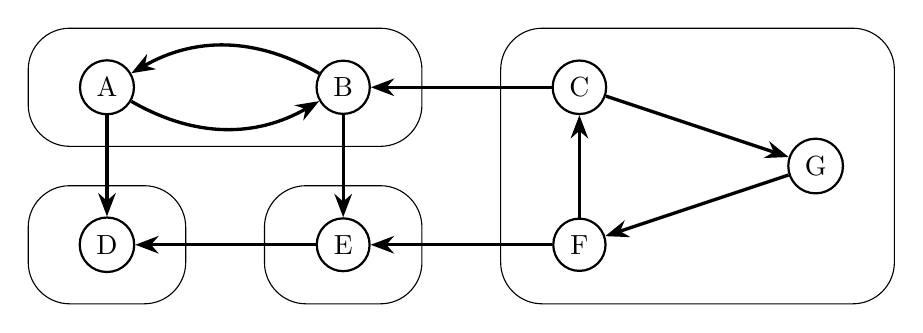
\begin{tikzpicture}
	\begin{scope}[every node/.style = {circle, thick, draw},
		every label/.append style={font = \small}]
		\node (A) at (0,0) {A};
		\node (B) at (3,0) {B};
		\node (C) at (6,0) {C};
		\node (D) at (0,-2) {D};
		\node (E) at (3,-2) {E};
		\node (F) at (6,-2) {F};
		\node (G) at (9,-1) {G};
	\end{scope}
	\begin{scope}[>={Stealth[black]},
			every edge/.style={draw=black, very thick}]
		\path [->] (A) edge[bend right=30] (B);
		\path [->] (A) edge (D);
		\path [->] (B) edge[bend right=30] (A);
		\path [->] (B) edge (E);
		\path [->] (C) edge (B);
		\path [->] (C) edge (G);
		\path [->] (F) edge (C);
		\path [->] (F) edge (E);
		\path [->] (G) edge (F);
		\path [->] (E) edge (D);
	\end{scope}
	\draw[rounded corners=15pt] (-1,-0.75) rectangle ++(5,1.5);
	\draw[rounded corners=15pt] (-1,-2.75) rectangle ++(2,1.5);
	\draw[rounded corners=15pt] (2,-2.75) rectangle ++(2,1.5);
	\draw[rounded corners=15pt] (5,-2.75) rectangle ++(5,3.5);

\end{tikzpicture}
\end{figure}
\vspace{-5 pt}
\subsubsection*{Explanation}
Let's look at why this algorithm works. 

Firstly, we have to take into account that the SCCs of a graph $G$ are preserved when 
we reverse all the edges and get $G^t$. The only relevant issue is the order in which
we process the SCCs. Let's assume we have a graph that has two SCC's:
\begin{figure}[h!]
	\centering
	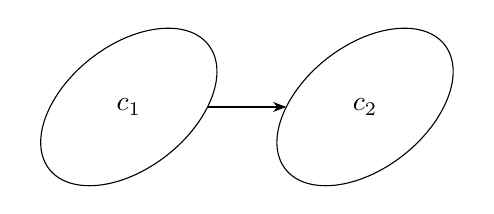
\begin{tikzpicture}
	\path[draw] plot [smooth cycle,tension=1]  coordinates 
		{(0,0) (1.5,1) (2,0) (0.5,-1)};
	\node (p1) at (1,0){$c_1$};
	
	\path[draw] plot [smooth cycle,tension=1]  coordinates 
		{(3,0) (4.5,1) (5,0) (3.5,-1)};
	\node (p1) at (4,0){$c_2$};

	\begin{scope}[>={Stealth[black]},
			every edge/.style={draw=black}]
		\path[->, ] (2,0) edge (3,0);
	\end{scope}

	\end{tikzpicture}
\end{figure}
We have three options:
\begin{itemize}
	\def\itemsep{0pt}
	\item \emph{They are not connected}. In this case, it does not matter
		whether we explore one or the other first since DFS will not 
		\say{leak} from one of them to the other
	\item \emph{They are connected only in one direction}. This is 
		the case that the figure shows and it is the most important one.
		If we explore $c_2$ before exploring $c_1$, DFS will first
		explore the entirety of $c_2$ and then, when it is exploring
		$c_1$ it will not \say{leak} to $c_2$ because those nodes are already
		marked as visited.
	\item \emph{They are connected in both directions}. This can never happen
		since, if they were to be connected bidirectionally, they would 
		form a single SCC, not two.
\end{itemize}
\newpage
Therefore, the correctness of this algorithm simply depends on exploring the SCCs in the 
right order.

Let's demonstrate the following claim: 
\vspace{-5pt}
\begin{center}
	\itshape
	In the previous setting, the maximum closing time of the nodes in $c_1$ will
	be greater than the maximum closing time of the nodes in $c_2$
\end{center}
We just have to distinguish two cases:
\begin{itemize}
	\item
	If we started exploring $c_2$ before $c_1$, there is no way to get to $c_1$ from
	$c_2$. Therefore, we will start exploring $c_1$ when we have already closed $c_2$,
	which means that all nodes in $c_2$ will be closed before the nodes in $c_1$
	are even \say{opened}.
	\item
	If we started exploring $c_1$ before $c_2$, at some point, DFS will leak to 
	$c_2$ and it will explore it entirely before returning to $c_1$. Therefore,
	the closing time of every node in $c_2$ will be lower than the closing time
	of the node where DFS was started in $c_1$.
\end{itemize}
This completes the proof of that statement. Let's now apply it to check the correctness 
of this algorithm using induction. 

\begin{itemize}
	\item \textit{Base case:}

After reversing the graph, we start with the node that was closed the last ($a$). Let's call
it's SCC $s_1$. Let's assume that there is an edge from $s_1$ to another SCC ($s_\alpha$) in
$G^t$, which would make DFS leak to that SCC. However, if that was the case, there
would be an edge from $s_\alpha$ to $s_1$ in $G$ and, therefore, we can apply the 
previous claim. 

In that scenario, the maximum closing time of  $s_\alpha$ would be greater than the maximum
closing time of $s_1$. This is a contradiction because we have stated that $a\in s_1$ 
is the node that was closed the last.

Therefore, there cannot be any edge from $s_1$ to another SCC.

\item \textit{Inductive step:}

	Let's now assume that we have already processed $n$ SCCs. We now choose a node $b$,
	which is the node with the highest closing time such that $b \not \in s_i, \
	i=1,\dots n$. 
	
	We will call the SCC of this node $s_{n+1}$.
	As before, we want to prove that $s_{n+1}$ is not 
	connected to any $s_\beta$ that hasn't been explored yet in $G^t$.

	We will assume that there is an edge from $s_{n+1}$ to a $s_{\beta}\not \in 
	\{s_1\dots s_n\}$. Therefore, in $G$, there is an edge from $s_{\beta}$ to
	$s_{n+1}$, which implies that the maximum closing time of $s_{\beta}$ is higher than
	the maximum closing time of $s_{n+1}$. 

	Let's define $x_\beta:=$( the node with the maximum closing time of $s_\beta$ ). 
	We just stated that the closing time of $x_\beta$ is greater than the closing time 
	of $b$ (there cannot be a node with a greater closing time in $s_{n+1}$).

	However, this is a contradiction. Therefore, $s_{n+1}$ cannot
	be connected to an $SCC$ that has not been explored and, thus, DFS will not leak.
	\\ \null \hfill $\qedsymbol$
\end{itemize}

\newpage
\cppcode[firstline=20]{code/graph/Kosaraju.cpp}
\noindent \textbf{\boldmath Running time: $\mathcal{O}(V+E)$}
\\ {\small (V = vertices, E = edges)}

\subsubsection*{Remarks}
\begin{itemize}
	\item The SCCs of any graph form a DAG
\end{itemize}

\newpage
\section{Kruskal's}
Kruskal's algorithm finds a minimum spanning forest of the given graph. To do so, it
uses UFDS to keep track of which nodes are already connected.
\subsection{UFDS}
UFDS (Union-find data structure) is a data structure that stores a partition of 
the vertices into sets such that all vertices in the same set are connected.
Each node $u$ will have two properties:
\begin{itemize}
	\setlength\itemsep{0pt}
	\item \textit{Parent}. It is the representative of the partition that
		contains $u$.
	\item \textit{Rank}. It is an upper bound of the height of the \say{tree}
		that starts on $u$. 
\end{itemize}
\cppcode[firstline=20]{code/graph/ufds.cpp}
\noindent \textbf{\boldmath Running time: $\mathcal{O}(E\log V)$}
\\ {\small (V = vertices, E = edges)}
\subsubsection{Explanation}
There are two main optimizations that are applied in this implementation:
\begin{itemize}
	\item \textit{Union by rank}. When we join two partitions, we have to choose
		a node to represent the new partition. In order to choose between the 
		two parents, we use their rank. 

		Our goal is to minimize the height of the trees that start at every node.
		Therefore, we pick the node with the highest rank as the parent. This 
		choice ensures that the rank of both parents will not increase. 

		However, if both parents have the same rank, we can choose either of 
		them.
	\item \textit{Path shortening}. The \texttt{find} function updates the value 
		of the parent of each node so that it does not point to it's 
		\say{immediate} parent but to the highest possible ancestor. This
		difference increases the efficiency of subsequent executions of the 
		\texttt{find} routine. 
\end{itemize}

\subsection{Kruskal's}
Using UFDS, the implementation of Kruskal is trivial. We just edges that connect 
vertices that are not connected already until all vertices are connected.
\cppcode[firstline=20]{code/graph/kruskal.cpp}
\noindent \textbf{\boldmath Running time: $\mathcal{O}(\max\{E,V\}\log(\max\{E,V\}) )$}
\\ {\small (V = vertices, E = edges)}

\newpage
\section{Flows and cuts}
In this section we will consider graphs as networks of pipes and the \say{weights}
of the edges will be their capacity.

\subsection{Edmonds-Karp's (Max Flow)}
The first problem that we have to consider is how to find the maximum flow from one
source node to a sink node. Edmonds-Karp's is an implementation of Ford-Fulkerson's 
that solves this problem.

This algorithm has some major caveats: it requires the use of an adjacency matrix
and it is not as fast as other options.

To improve its running time, this implementation uses both an adjacency matrix 
and adjacency list. However, we have to be careful when creating the adjacency
list since for every forward edge, we need a backward edge that will start with 
a capacity of 0 but its capacity may increase. 

Therefore, the code for adding edges would be the following:
\begin{minted}{cpp}
// Add a directed edge
void addedgeUni(int orig, int dest, ll flow) {
    adjList[orig].pb(dest);
    adjMat[orig][dest] = flow;
    adjList[dest].pb(orig);   //Add edge for residual flow
}
// Add a bidirectional edge
void addEdgeBi(int orig, int dest, ll flow) {
    adjList[orig].pb(dest);
    adjList[dest].pb(orig);
    adjMat[orig][dest] = flow;
    adjMat[dest][orig] = flow;
}
\end{minted}
\newpage
\cppcode[firstline=20,lastline=63]{code/graph/edmonds-karp.cpp}
\noindent \textbf{\boldmath Running time: $\mathcal{O}(VE^2)$}
\\ {\small (V = vertices, E = edges)}
\subsubsection{Remarks}
\begin{itemize}
	\item If we have multiple sources $s_1,\dots, s_n$ and multiple sinks 
		$t_1,\dots t_n$, we can use the same algorithm. We just have to create a 
		source $s$ that connects to $s_i$ with edges of infinite capacity and
		a sink $t$ such that $s_i$ is connected to $t$ with edges of infinite
		capacity.
		
	\item If we have vertex capacities, we can split the vertex $v$ into two vertices:
		$v_{in}$ and $v_{out}$, connected with an edge that has the vertex 
		capacity as a capacity. Then we connect the incoming edges to $v_{in}$ and 
		the out-coming edges to $v_{out}$


\end{itemize}

\chapter{Mathematics}

\section{General calculations}
\subsection{Binary exponentiation}
Binary exponentiation calculates a power in logarithmic 
time. Furthermore, it can be used for modular arithmetic:
\cppcode[firstline=20,]{code/maths/binary_exp.cpp}
\noindent \textbf{\boldmath Running time: $\mathcal{O}(\log(\mathrm{exp}))$}


\newpage
\section{Modular arithmetic}
\subsection{Inverses}
To calculate a modular inverse, we will use Fermat's little theorem:
\[
	a^{p-1}\equiv 1 \ \mathrm{mod} \ p  \ \implies \  a^{p-2}\equiv a^{-1} \ \mathrm{mod} p
\]
If we combine this fact with binary exponentiation, we can obtain the 
modular inverse in logarithmic time:
\begin{minted}{cpp}
ll inverse(ll num) {
    return power(num, mod - 2);
}
\end{minted}
\noindent \textbf{\boldmath Running time: $\mathcal{O}(\log(\mathrm{mod}))$}

\section{Catalan numbers}
We define the nth Catalan number as:
\[
	C_n= \frac{1}{n+1}{2n\choose n} = \frac{1}{n+1}\frac{(2n)!}{n! \;n!}
\]
We can also define them recursively:
\[
	C_0 = 1 \qquad C_{n+1} = \sum_{i=0}^n\big (C_i \; C_{n-i}\big)
\]
They can be used to solve many different problems. For instance:
\begin{itemize}
	\item Number of different binary trees of $n$ nodes. We can look
		at the specific case $n=3$. As we can see in the figure below,
		$C_3=5$. Furthermore, we can clearly identify the recursive relationship:
		\[
			C_3= (\text{3 is root}) + (\text{2 is root}) + (\text{1 is root}) = C_2\cdot C_0 + 
			C_1\cdot C_1 + C_0\cdot C_2
		\]
		\begin{figure}[h!]
			\centering
			\scalebox{0.5}{
			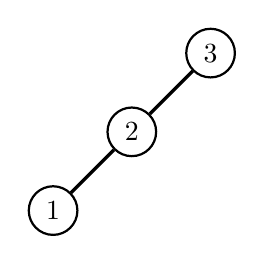
\begin{tikzpicture}
				\begin{scope}[every node/.style = {circle, thick, draw},
					every label/.append style={font = \small}]
					\node (A) at (0,0) {3};
					\node (B) at (-1,-1) {2};
					\node (C) at (-2,-2) {1};
				\end{scope}
				\begin{scope}[>={Stealth[black]},
						every edge/.style={draw=black, very thick}]
					\path [-] (A) edge (B);
					\path [-] (B) edge (C);
				\end{scope}
			\end{tikzpicture}
			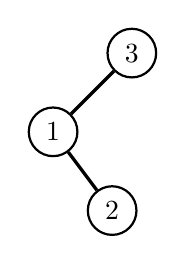
\begin{tikzpicture}
				\begin{scope}[every node/.style = {circle, thick, draw},
					every label/.append style={font = \small}]
					\node (A) at (0,0) {3};
					\node (B) at (-1,-1) {1};
					\node (C) at (-0.25,-2) {2};
				\end{scope}
				\begin{scope}[>={Stealth[black]},
						every edge/.style={draw=black, very thick}]
					\path [-] (A) edge (B);
					\path [-] (B) edge (C);
				\end{scope}
			\end{tikzpicture}

			\hspace*{60 pt}

			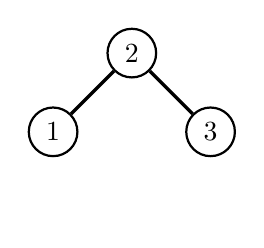
\begin{tikzpicture}
				\begin{scope}[every node/.style = {circle, thick, draw},
					every label/.append style={font = \small}]
					\node (A) at (0,0) {2};
					\node (B) at (1,-1) {3};
					\node (C) at (-1,-1) {1};
				\end{scope}
					\node (J) at (-1,-2) {};
				\begin{scope}[>={Stealth[black]},
						every edge/.style={draw=black, very thick}]
					\path [-] (A) edge (B);
					\path [-] (A) edge (C);
				\end{scope}
			\end{tikzpicture}
			\hspace*{30 pt}
			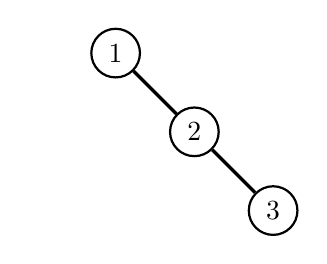
\begin{tikzpicture}
				\begin{scope}[every node/.style = {circle, thick, draw},
					every label/.append style={font = \small}]
					\node (A) at (0,0) {1};
					\node (B) at (1,-1) {2};
					\node (C) at (2,-2) {3};
				\end{scope}
					\node (J) at (-1,-2) {};
				\begin{scope}[>={Stealth[black]},
						every edge/.style={draw=black, very thick}]
					\path [-] (A) edge (B);
					\path [-] (B) edge (C);
				\end{scope}
			\end{tikzpicture}
			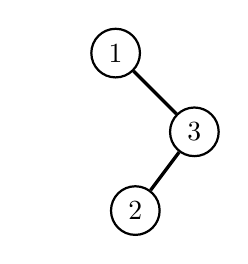
\begin{tikzpicture}
				\begin{scope}[every node/.style = {circle, thick, draw},
					every label/.append style={font = \small}]
					\node (A) at (0,0) {1};
					\node (B) at (1,-1) {3};
					\node (C) at (0.25,-2) {2};
				\end{scope}
					\node (J) at (-1,-2) {};
				\begin{scope}[>={Stealth[black]},
						every edge/.style={draw=black, very thick}]
					\path [-] (A) edge (B);
					\path [-] (B) edge (C);
				\end{scope}
			\end{tikzpicture}
	}
	\end{figure}
\end{itemize}


\chapter{Geometry}

\section{Area of polygon}

\begin{wrapfigure}{r}{0.5\linewidth}
	\centering
	\resizebox{80 mm}{!}{\import{./Figures/}{geometry_area.pdf_tex}}
	\vspace*{-40 pt}
\end{wrapfigure}

In this problem, we are given a polygon expressed as a list of vertices.
We are tasked with calculating the area of the polygon.

For now, we will assume that the points are ordered in a clock-wise fashion
and we will consider three different scenarios for each segment:
\begin{itemize}
	\item $\Delta x=0$. It does not add any area to the polygon.
	\item $\Delta x\ne 0$. It has an area associated with it that is equal
		to the area between the segment and the $x$ axis
		\begin{itemize}
			\item $\Delta x > 0$. We consider this area positive
				(green on the figure)
			\item $\Delta x < 0$. We consider this area negative
				(red on the figure)
		\end{itemize}
\end{itemize}

Now we add all the areas associated with each segment and we get a total area.
If the vertices were ordered in a counter-clock-wise fashion, this total
area will be negative. Therefore, we will only consider the absolute
value of the result.
\cppcode[firstline=20,lastline=63]{code/geometry/polygon_area.cpp}
\noindent \textbf{\boldmath Running time: $\mathcal{O}(n)$}
\\ {\small (n = vertices)}




\end{document}
